\begin{center}
	{\Large\bf 《高等数学》秋季学期期中测验}
	
	(闭卷考试,时间:150分钟)
\end{center}

{\bf 一、填空题(每题3分)}

1.\;曲线$y=(x+2)e^{-x}$的拐点为\underline{\hspace{4cm}}.
\bs

2.\;$\limx{\pi}\df{\cos\frac x2}{e^{\sin x}-e^{\sin4x}}=$
\underline{\hspace{4cm}}.
\bs

3.\;$f(x)=xe^{2x}$的$100$阶带Peano余项的Maclaurin公式为
\underline{\hspace{4cm}}.
\bs

4.\;$f(x)=x^3+2x^2+4x\,(x>0)$,$g(x)$为其反函数,则$g'(7)=$
\underline{\hspace{4cm}}.
\bs

5.\;$f(x)$是以$5$为周期的连续函数,且在原点附近满足
$$f(1+\sin x)-3f(1-\sin x)=8x+\circ(x),$$
已知$f(x)$在$x=1$可导,则$y=f(x)$在$x=6$处的切线斜率为
\underline{\hspace{4cm}}.
\bs

{\bf 二、选择题(每题3分)}

1.\;函数$f(x)$在$x=0$处可导,则$\limx0\df{f(x)e^x-f(0)}{x}=$(\quad)%D
\begin{tabbing}
	\hspace{8cm}\=\kill
	\quad\quad\quad(A)\;$f(0)$ \> 
	(B)\;$f'(0)$ \\ 
	\quad\quad\quad(C)\;$f'(0)-f(0)$\>
	(D)\;$f'(0)+f(0)$
\end{tabbing}

2.\;设函数$y=f(x)$满足:对所有$x$有$f'(x)<0$,当$|x|>1$时,
$f''(x)>0$,当$|x|<1$时,$f''(x)<0$,并且$\limx{\infty}[f(x)+x]=0$,
则下列可能是$y=f(x)$的图像的是
(\quad)%A
\begin{center}
	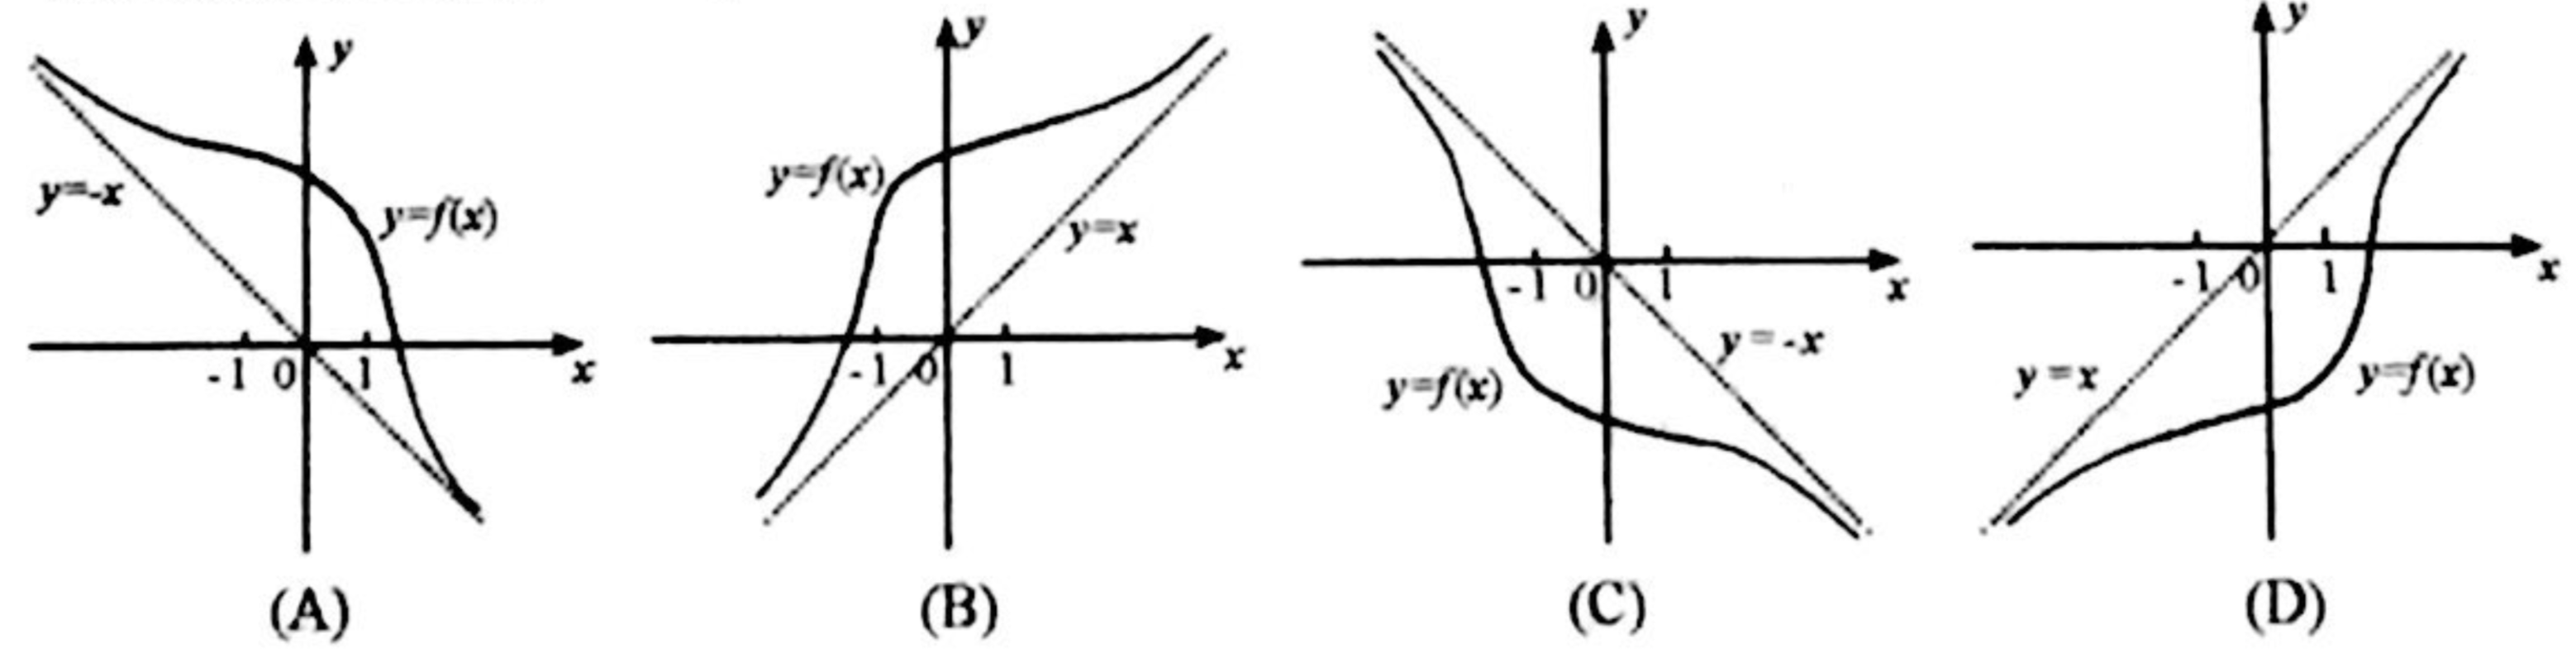
\includegraphics[width=\textwidth]{./UnitTest/images/abcd.pdf}
\end{center}

3.\;$f(x)\left\{\begin{array}{ll}
	x^{\frac53}\sin\df1x, & x\ne 0\\ 0, & x=0
\end{array}\right.$在$x=0$处(\quad)%
\begin{tabbing}
	\hspace{8cm}\=\kill
	\quad\quad\quad(A)\;不连续 \> 
	(B)\;连续但不可导 \\ 
	\quad\quad\quad(C)\;可导但导函数不连续\>
	(D)\;导函数连续
\end{tabbing}

4.\;函数$f(x)=\ln|x-1|$的导数是(\quad)%B
\begin{tabbing}
	\hspace{8cm}\=\kill
	\quad\quad\quad(A)\;$\df1{|x-1|}$ \> 
	(B)\;$\df1{x-1}$ \\ 
	\quad\quad\quad(C)\;$\df1{1-x}$\>
	(D)\;$\left\{\begin{array}{ll}
	\df1{x-1},&x>1\\ \df1{1-x},&x<1
	\end{array}\right.$
\end{tabbing}

5.\;$f(x)=(1-e^x)|x^3-x|$的不可导点个数为(\quad)%B

\quad (A)\;$0$\quad\quad\quad(B)\;$1$
\quad\quad\quad (C)\;$2$\quad\quad\quad(D)\;$3$

\bigskip

{\bf 三(6分)}、计算极限$\limx0\df{x-\sin x}{\sqrt{1+x^2\tan x}-1}$。

\bs

{\bf 四(6分)}、计算极限$\limx0\left[\df{(1+x)^{\frac1x}}{e}\right]^{\frac1x}$。

\bs

{\bf 五(6分)}、求曲线$y=x+\df{\sin x}{x+x^2}$的渐近线。

\bs

{\bf 六(6分)}、设$f(x)$在$(-\infty,+\infty)$上处处二阶可导,
且$f''(x)>0$,$\limx0\df{f(x)}x=1$,证明:对任意$x\in(-\infty,+\infty)$,
恒有$f(x)\geq x$。

\bs

{\bf 七(6分)}、证明:$x>0$时,总有$x(2+\cos x)>3\sin x$。

\bs

{\bf 八(8分)}、设$f(x)=\left\{\begin{array}{ll}
	\df{\ln(1+x)}x, & x>0,\\ a+b\cos x, & x\leq 0
\end{array}\right.$,问是否存在$a,b$使得$f(x)$处处可导。

\bs

{\bf 九(8分)}、流星是一种常见的天文现象。它是由空间物体进入大气层后,
与大气摩擦发热燃烧而形成的。流星落至地面时残留的物质称为陨石。假设一半径为$R_0$
的球状空间物体,进入大气层后其体积减少的速率与半径$r$的平方成正比,比例常数
$a>0$,且燃烧过程中其始终保持球状。已知该物体经过时间$T$后落到地面,所
行程的陨石半径为$r_0(<R_0)$。
\begin{enumerate}[(1)]
  \setlength{\itemindent}{1cm}
  \item 求燃烧过程中该物体的半径$r$关于时间$t$的变化率;
  \item 推导$R_0$关于$T$和$r_0$的表达式。
\end{enumerate}

% 设$f(x)$在$(-\infty,+\infty)$上可微,且为奇函数。
% \begin{enumerate}[(1)]
%   \setlength{\itemindent}{1cm}
%   \item 对任意$b>0$,存在$c\in(0,b)$,使得$(c-b)f'(c)+f(c)=0$;
%   \item 是否存在$d\in(-b,0)$,使得$(d+b)f'(d)+f(d)=0$?其中
%   $d$与$c$有何关系?请说明理由。
% \end{enumerate}

\bs

{\bf 十(8分)}、设$f(x)$在$x=0$处二阶可导,且$\limx0\df{\sin x-xf(x)}{x^3}=1$,
求$y=f(x)$在$x=0$处的曲率。

\bs

{\bf 十一(8分)}、设$0<a<b$,证明不等式:$\df{2a}{a^2+b^2}<
\df{\ln b-\ln a}{b-a}<\df1{\sqrt{ab}}$。

\bs

{\bf 十二(8分)}、$f(x)$在$[-1,1]$上有三阶连续导函数,$f(-1)=0$,
$f(1)=1$,$f'(0)=0$,证明:存在$\xi\in(-1,1)$,使得$f'''(\xi)=3$。

\newpage

\begin{center}
	{\Large\bf 解答与评分标准}\ps{\b 1.若解法与参考答案不同,参照本评分标准的特点分段给分\\
	2.计算题只写结果,缺少计算过程,最多得1分}
\end{center}

{\bf 一、填空题(每题3分)}

1.\;$(0,2)$\quad\quad 
2.\;$\df1{10}$\quad\quad
3.\;$\sum\limits_{k=0}^{99}\df{2^k}{k!}x^{k+1}+\circ(x^{100})$\quad\quad
4.\;$\df1{10}$\quad\quad
5.\;$2$

[提示]:
2.$\mbox{原式}=\limx{\pi}\df{\cos\frac x2}{\sin x-\sin 4x}
=\limx{\pi}\df{-\frac12\sin\frac x2}{\cos x-4\cos 4x}=\df1{10}$

4.$x=1$时$f(x)=7$,故$g'(7)=\df1{f'(1)}=\df1{10}$.

5.显然$f(1)=0$,
\begin{align*}
	8&=\limx0\df{f(1+\sin x)-3f(1-\sin x)}{x}\\
	&=\limx0\df{f(1+\sin x)-f(1)}{\sin x}\df{\sin x}x
	+3\limx0\df{f(1-\sin x)-f(1)}{-\sin x}\df{\sin x}x\\
	&=4f'(1)=4f'(6).
\end{align*}

{\bf 二、选择题(每题3分):}\quad D\quad A\quad C\quad B\quad C

[提示]:1.
$$\mbox{原式}=\limx0\df{f(x)-f(0)}{x}\limx0e^x
+f(0)\limx0\df{e^x-1}x=f'(0)+f(0).$$


{\bf 三(6分)、}解:
\begin{align*}
	\mbox{原式}&=\limx0\df{x-\sin x}{x^2\tan x}\\
	&=\limx0\df{x-\sin x}{x^3}\tag{+2\mbox{\;分}}\\
	&=\limx0\df{1-\cos x}{3x^2}\tag{+2\mbox{\;分}}\\
	&=\limx0\df{\frac{x^2}2}{3x^2}=\df16.\tag{+2\mbox{\;分}}
\end{align*}
\fin

{\bf 四(6分)、}解:
\begin{align*}
	\mbox{原式}&=\exp\left[\limx0\df{\ln(1+x)-x}{x^2}\right]\tag{+2\mbox{\;分}}\\
	&=\exp\left[\limx0\df{\df1{1+x}-1}{2x}\right]\tag{+2\mbox{\;分}}\\
	&=e^{-\frac12}.\tag{+2\mbox{\;分}}
\end{align*}
\fin

{\bf 五(6分)、}解:显然
$$\limx{-1}y=\limx{-1}\left[x+\df{\sin x}{x(x+1)}\right]=\infty,$$
故$x=-1$为铅直渐近线。\hfill{(+2\;分)}

又
$$\limx{\infty}\df yx=\limx{\infty}\left[1+\df{\sin x}{x^2(x+1)}\right]=1,$$
且
$$\limx{\infty}(y-x)=\limx{\infty}\df{\sin x}{x(x+1)}=0,$$
故$y=x$为斜渐近线。\hfill{(+4\;分)}$\Box$

\bs

{\bf 六(6分)、}证:由已知可得$f(0)=0$,进而$\limx0\df{f(x)-f(0)}x
=\limx0\df{f(x)}x=1$,也即$f'(0)=1$。\hfill{(+2\;分)}

设$F(x)=f(x)-x$,则由已知$F(0)=0,F'(0)=0$。
注意到$F''(x)=f''(x)>0$,故当$x>0$时,$F'(x)>0$;\hfill{(+2\;分)}

进而可知当$x>0$时,$F(x)>0$,即证。\hfill{(+2\;分)}$\Box$

\bs

{\bf 七(6分)、}证:结论中的不等式即为$\df{3\sin x}{2+\cos x}<x$。\hfill{(+1\;分)}

令$f(x)=x-\df{3\sin x}{2+\cos x}$,则
$$f'(x)=\df{(1-\cos x)^2}{(2+\cos x)^2}\geq 0.\eqno{(+3\;\mbox{分})}$$
显然$f'(x)$在$[0,+\infty)$的任何子区间内不恒为零,故$f(x)$当$x\geq 0$时
严格单调递增,又$f(0)=0$,故当$x>0$时,$f(x)>0$,即证。\hfill{(+2\;分)}$\Box$

\bs

{\bf 八(8分)、}解:显然当$x\ne0$时,$f(x)$可导。
假设$f'(0)$存在,则$f(x)$在$x=0$处连续,也即
$f(0+0)=f(0-0)=f(0)$,进而可得$a+b=1$。\hfill{(+2\;分)}

又
\begin{align*}
	f'_-(0)&=\limx{0^-}\df{a+b\cos x-(a+b)}x=0,\tag{+1\mbox{\;分}}\\
	f'_+(0)&=\limx{0^+}\df{\df{\ln(1+x)}x-1}x=-\df12,\tag{+3\mbox{\;分}}\\
\end{align*}
故$f'_-(0)\ne f'_+(0)$,从而可知假设错误,故不存在$a,b$能够使得$f(x)$处处可导。
\hfill{(+2\;分)}$\Box$

\bs

{\bf 九(8分)、}解:(1)设物体燃烧时间$t$后,所剩体积为$V(t)$,则
$$V(t)=\df43\pi r^3(t)
\quad\Rightarrow\quad
V'(t)=4\pi r^2(t)r'(t).\eqno{(+2\;\mbox{分})}$$
又由已知$V'(t)=-ar^2(t)$,从而可得$r'(t)=-\df{a}{4\pi}$。\hfill{(+2\;分)}

(2)由(1)的结论,可得$r(t)=-\df{at}{4\pi}+C$。\hfill{(+2\;分)}

因$r(0)=R_0$,故
$$r(t)=-\df{at}{4\pi}+R_0.$$
由已知时间$T$后半径为$r_0$,也即$r_0=-\df{aT}{4\pi}+R_0$,故
$$R_0=r_0+\df{aT}{4\pi}.\eqno{(+2\;\mbox{分})}$$
\fin

{\bf 十(8分)、}解:由Taylor公式,
\begin{align*}
	\limx0\df{\sin x-xf(x)}{x^3}
	&=\limx0\df{x-\frac{x^3}6+\circ(x^3)-x\left[
	f(0)+f'(0)x+\frac{f''(0)}2x^2+\circ(x^2)\right]}{x^3}\\
	&=\limx0\df{[1-f(0)]x-f'(0)x^2-\left[\frac16+\frac{f''(0)}2x^3\right]}
	{x^3}=1,\tag{+3\mbox{\;分}}
\end{align*}
从而可知
$$f(0)=1,\quad f'(0)=0,\quad f''(0)=-\df73.\eqno{(+2\;\mbox{分})}$$
进而由曲率公式
$$K=\df{|f''(0)|}{\{1+[f'(0)]^2\}^{\frac32}}=\df73.\eqno{(+3\;\mbox{分})}$$
\fin

{\bf 十一(8分)、}证:先证左端不等式:由Lagrange中值定理,存在$\xi\in(a,b)$,使得
$$\df{\ln b-\ln a}{b-a}=\df1{\xi}>\df1b>\df{2a}{a^2+b^2}.\eqno{(+3\;\mbox{分})}$$

再证右端不等式:令$f(x)=\ln x-\ln a-\df{x-a}{\sqrt{ax}}$,则当$x>a$时,
$$f'(x)=-\df{(\sqrt x-\sqrt a)^2}{2x\sqrt{ax}}<0,\eqno{(+2\;\mbox{分})}$$
又$f(a)=0$,由此可知对任意$x>a$,总有$f(x)<f(a)=0$,也即
$$\ln x-\ln a<\df{x-a}{\sqrt{ax}},\eqno{(+3\;\mbox{分})}$$
令$x=b$,即证。\fin

{\bf 十二(8分)、}证:由Taylor公式,存在$\xi_1\in(-1,0),\xi_2\in(0,1)$,使得
\begin{align*}
	0&=f(-1)=f(0)-f'(0)+\df12f''(0)-\df16f'''(\xi_1),\tag{+2\mbox{\;分}}\\
	1&=f(1)=f(0)+f'(0)+\df12f''(0)+\df16f'''(\xi_1).\tag{+2\mbox{\;分}}
\end{align*}
以上两式相减,可得
$$1=2f'(0)+\df16[f'''(\xi_1)+f'''(\xi_2)]
\quad\Rightarrow\quad
f'''(\xi_1)+f'''(\xi_2)=6.\eqno{(+2\;\mbox{分})}$$
由已知$f'''(x)$为连续函数,故由介值定理,存在$\xi\in(\xi_1,\xi_2)\subset(-1,1)$,
使得
$$f'''(\xi)=\df12[f'''(\xi_1)+f'''(\xi_2)]=3.\eqno{(+2\;\mbox{分})}$$
即证。\fin
